\documentclass[tikz,border=2pt]{standalone}
\usepackage{amsmath}
\usepackage{amssymb}
\usepackage{xcolor}

\definecolor{journalink}{HTML}{1F1C18}
\definecolor{journalmuted}{HTML}{8A7F72}
\definecolor{journalaccent}{HTML}{9C2D2D}

\begin{document}
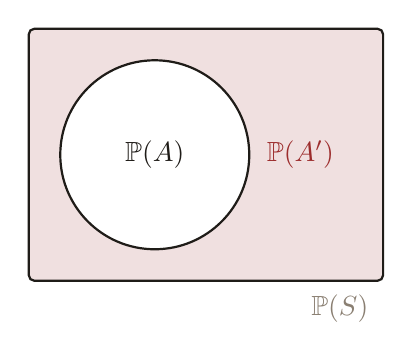
\begin{tikzpicture}[
  x=1cm,
  y=1cm,
  every node/.style={font=\normalsize}
]
  \def\circleA{(0,0) circle (1.2)}

  \begin{scope}[even odd rule]
    \clip \circleA (-1.6,-1.6) rectangle (2.9,1.6);
    \path[fill=journalaccent, fill opacity=0.15, rounded corners=2pt] (-1.6,-1.6) rectangle (2.9,1.6);
  \end{scope}

  \draw[journalink, line width=0.8pt, rounded corners=2pt] (-1.6,-1.6) rectangle (2.9,1.6);
  \draw[journalink, line width=0.8pt] \circleA;

  \node[journalink] at (0,0) {$\mathbb{P}(A)$};
  \node[journalaccent] at (1.85,0) {$\mathbb{P}(A')$};
  \node[journalmuted] at (2.35,-1.95) {$\mathbb{P}(S)$};
\end{tikzpicture}
\end{document}
